\section{LSST Observing Cadence Optimization to Enhance PHA Completeness \label{sec:opsim}}

The effects of varying the LSST observing strategy on PHA completeness and other science can be evaluated in detail using a combination of the LSST Operations Simulator (OpSim) and the LSST Metrics Analysis Framework (MAF). 

The LSST Operations Simulation (OpSim) is a python software package that generates a realistic pointing history, with the time, filter, location, astronomical conditions, weather conditions, and predicted point-source 5-sigma limiting magnitude, for each LSST visit for ten years. This pointing history is generated using weather data (cloudiness and seeing) from the Cerro Pachon site and a high-fidelity model of the telescope itself (including slew and settle time and dome movement, for example), combined with a parameterized set of observing proposals that determine how the scheduling algorithm attempts to gather observations. By configuring OpSim with different parameters for the observing proposals, we can generate a series of simulated surveys which prioritize different science goals. 

The LSST Metrics Analysis Framework (MAF) is a user-oriented, python package for evaluating the pointing history from these simulated surveys in light of particular science goals or interests. The results of metrics coded in the MAF framework can be calculated for any given simulated survey and compared as proposal parameters are changed in OpSim. Metrics will be gathered from as wide a cross section of the astronomical community as possible, together with "figures of merit" that summarize and define 'success' for a given metric. This permits a thorough investigation of the trades between different observing strategies, in terms of the effect on science goals.

We can use MAF to evaluate the effect of various observing strategies on moving object completeness and characterization as well. Here we focus on discovery completeness of Potentially Hazardous Asteroids (PHAs) as both the observing strategy (related to changes in OpSim proposal parameters) and discovery criteria (related to LSST Data Management (DM) and the Moving Object Processing Software (MOPS) workloads) are varied. 

\subsection{Details of MAF analysis}

Using MAF to evaluate metrics for moving objects, such as PHAs, requires first defining the parameters of the input small body population by:

\begin{enumerate}
\item{Defining an orbital distribution for the input moving object population, specified by a set of orbital parameters for each object. Here we have chosen to use an orbital distribution defined by the large ($>1$ km) diameter known PHAs, as reported to the Minor Planet Center (MPC). This population is thought to be relatively complete and thus should be relatively unbiased. For comparison with other completeness estimates which use an Near Earth Object (NEO) population based on the \cite{Bottke2002} model instead of the subset of these objects which are classified as PHAs, we also evaluate completeness using a random sample of 2000 NEOs from the synthetic solar system model presented in \cite{Grav2011}.  A plot of the $a$, $e$, $i$ distribution for these PHAs and NEOs is shown in Figure~\ref{fig:PHA_orbits}.  }
\begin{figure}
\centering
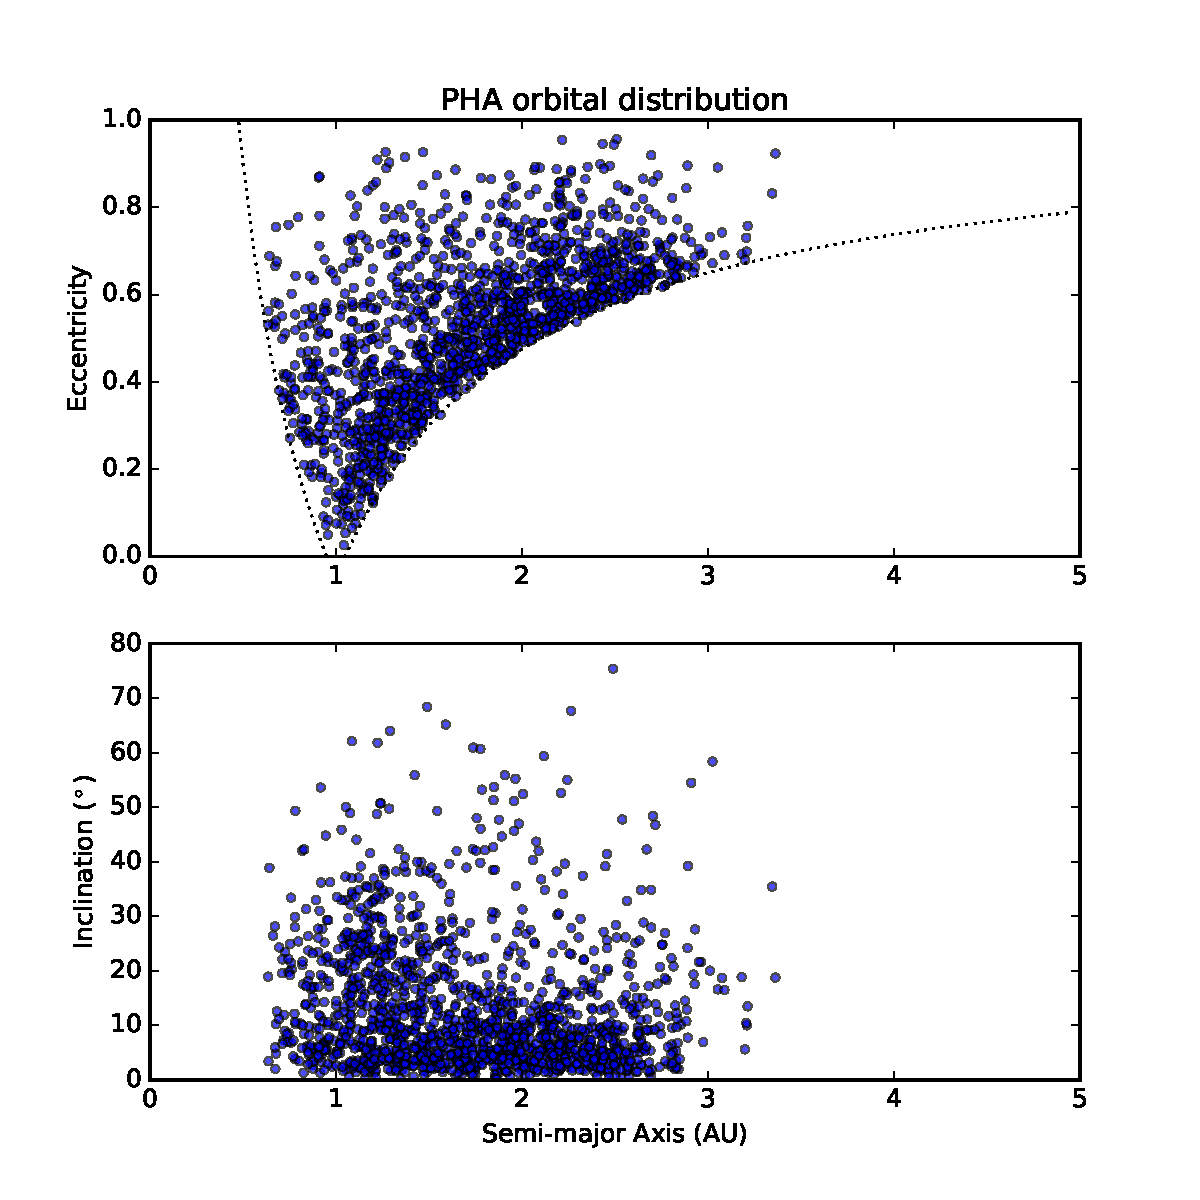
\includegraphics[width=0.45\textwidth]{figures/pha20141031_orbits} 
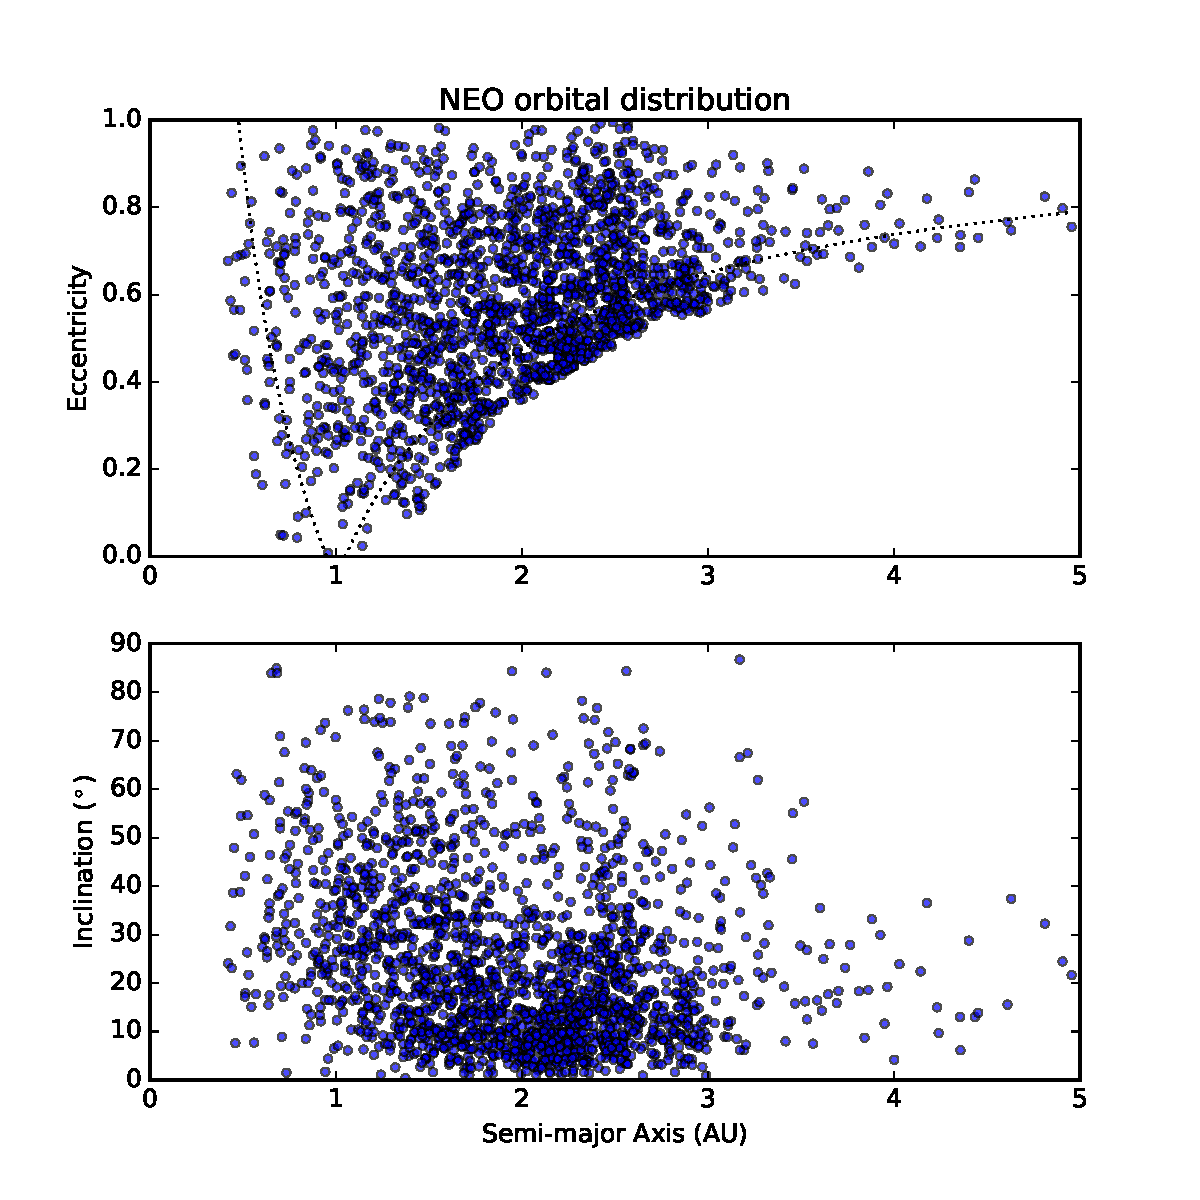
\includegraphics[width=0.45\textwidth]{figures/neos_2k_orbits}
\caption{The eccentricity and inclination distributions, as a function of semi-major axis, of the PHAs (left) and NEOs (right) used in this analysis. The PHA population consists of the orbital distribution of $>1$~km PHAs recorded by the MPC as of 2014 (1511 objects). The NEO population is a random sampling of 2000 NEOs from the S3M \citep{Grav2011}, a synthetic solar system model based on the \cite{Bottke2002} NEO orbital distribution. \label{fig:PHA_orbits}}
\end{figure}

\item{Optionally, define a size for each object. For populations where the size distribution is strongly tied to the orbital distribution, this is necessary. However, most small body populations can be well described by independent orbital and size distributions; the PHA population larger than 140~m in diameter can be generally described in this manner. In these cases, a smaller set of orbits can be used to represent the overall larger population; during analysis, each object can be `cloned' from a fiducial $H$ magnitude associated with the orbit to a range of $H$ magnitudes covering the range interesting for analysis. This makes the metric analysis, and particularly the generation of the expected observations for each object, simpler and faster. As long as sufficient resolution of the orbital parameter space is maintained, the metric results over the range of $H$ magnitudes will be comparable to the results calculated with a larger population. Here we use the small population of $>1$~km diameter known PHAs and clone them to a range of $H$ magnitudes between $H$=11 and $H$=28. We have verified with a larger, simulated set of NEOs that reducing the population from 10,000 model NEOs to 2000 model NEOs does not change the calculated survey  completeness. }

\item{Optionally, define a spectrum or color for each object. This facilitates the conversion from $H$ magnitude (assumed to be in $V$ band) to the apparent magnitude in a given LSST observation, which may be in any of $u$, $g$, $r$, $i$, $z$, or $y$ filters. Here we have assumed that our entire PHA population consists of C-type asteroids, with resulting transformations to  LSST bandpasses as described in Table~\ref{tab:sed_colors}.  }
\begin{deluxetable}{ccccccc}
\centering
\tablecolumns{7}
\tablecaption{Color transformations from Harris $V$ band to LSST bandpasses, for C and S type asteroids. \label{tab:sed_colors}}
\tablewidth{0.7\textwidth}
\tablehead{ Type & $V-u$ & $V-g$ & $V-r$ & $V-i$ & $V-z$ & $V-y$  \\ }
\startdata
C  & -1.53 &  -0.28 &  0.18 &  0.29 &  0.30 & 0.30 \\
S & -1.82 &  -0.37 &  0.26 & 0.46 &  0.40 & 0.407  \\
\enddata
\end{deluxetable}

\end{enumerate}

Using the details of the input population, MAF then generates the expected observations of each object using the pointing history from a specific OpSim simulated survey. Ephemerides are generated using OpenOrb \citep{OpenOrb2009} for a closely spaced grid of times, and then interpolated to the exact times of each OpSim pointing. If the object is within the LSST field of view, its predicted position, velocity, and apparent $V$ magnitude (for the fiducial $H$ magnitude associated with the orbit) is recorded along with information about the simulated observation itself (such as the seeing, limiting magnitude, filter, and boresight RA/Dec). The full LSST camera footprint, including chipgaps, is used to determine if an object is within the field of view. The camera footprint is shown in Figure~\ref{fig:camera_footprint}. 

\begin{figure}
\centering
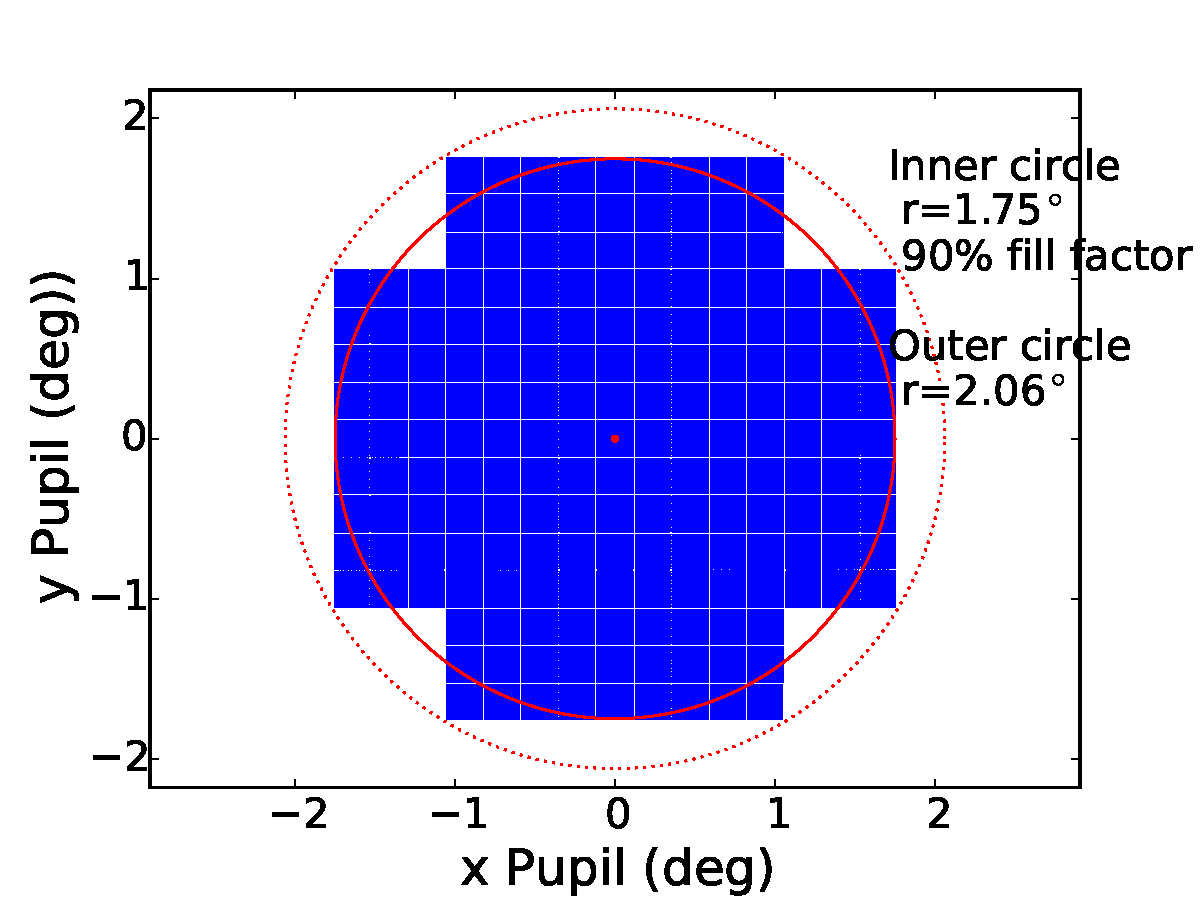
\includegraphics[width=0.65\textwidth]{figures/focalplane} 
\caption{Model of the LSST camera footprint, including chipgaps and CCD + raft layout. \label{fig:camera_footprint}}
\end{figure}

Trailing loss estimates are provided by MAF. Trailing losses occur whenever the motion of a moving object spreads its photons over a wider area than a simple stellar PSF. There are two aspects
of trailing loss to consider: simple SNR losses and detection losses.
The first is simply the degradation in SNR that occurs (relative to a
stationary PSF) because the trailed object includes a larger number of
background pixels in its footprint. This will affect photometry and
astrometry, but typically doesn't directly affect whether an object is
detected or not. The second effect (detection loss) is not related to
measurement errors but does typically affect whether an object passes
a detection threshhold. Detection losses occur because source
detection software is optimized for detecting point sources;
a stellar PSF-like filter is used when identifying sources that pass
above the defined threshhold, but this filter is non-optimal for
trailed objects. This can be mitigated with improved software ({\it                                                                               
e.g.} detecting to a lower SNR threshhold and attempting to detect
sources using a variety of trailed PSF filters). Both trailing losses can
be fit as:
\begin{eqnarray}
\Delta \, m & = &-1.25 \, log_{10} \left( 1 + \frac{a \, x^2} { 1 + b\,
    x} \right) \\
x & = & \frac{v \, T_{exp}} {24 \, \theta} 
\end{eqnarray}
where $v$ is the velocity (in degrees/day), $T_{exp}$ is the exposure
time (in seconds), and $\theta$ is the FWHM (in arcseconds). For
SNR trailing losses, we find $a = 0.67$ and $b = 1.16$; for
detection losses, we find $a=0.42$ and $b=0$. An illustration of the
magnitude of these trailing loss effects for 0.7'' seeing is given in
Figure~\ref{trailinglosses}. When considering whether a source would
be detected at a given SNR using typical source detection software,
the detection loss should be used.


and 'fading'

explain cloning and analysis (differential completeness), and how combined to generate cumulative completeness


\subsection{OpSim Simulated Surveys}

describe set of new opsim runs (minion1016, astrolsst011016, astrolsst011015, astrolsst011017)

and summarize completeness changes 
\begin{enumerate}
\item baseline (minion1016) to more observations in NES
\item adding two years to astrolsst011016
\item extending MOPS window to 30 days, at SNR=5
\item adding longer exposures throughout the ecliptic (astrolsst011015/astrolsst1017)
\item making DM find objects with trailing loss, not detection losses
\item extending SNR limit to 4 instead of 5
\end{enumerate}



\subsection{Systematic effects due to varying modeling assumptions}


\subsection{Comparison with external completeness analysis}

The leading systematic effects in completeness estimates are: 
\begin{enumerate}
\item NEO vs. PHA difference (the completeness is about $\sim$5\% higher for PHAs than for NEOs) 
\item Different sample definitions: $H<22$ vs. $D>140$m (as shown by \citep{GMS2016}, completeness
           increases by $\sim$5\% when $H$-based criterion is used) 
\item Variations of ``discovery window'' (e.g., X visit pairs in N nights: changing N from 15 to 30 with X=3 increases
          completeness by 3\%; changing X from 3 to 4 with N=15 decreases completeness by 6\%). 
\end{enumerate}          
          

\subsection{Remaining uncertainties in completeness estimates}

Common to all, really.          

\begin{enumerate}
=======
\item Orbital parameter distribution for the simulated asteroid population (e.g. the Bottke model
             vs. the Granvik model); varying populations contribute completeness uncertainty of about a few percent) 
\item Variations of the ``discovery window'' (e.g., X visit pairs in N nights: changing N from 15 to 30 with X=3 increases
          completeness by about 4\%; changing X from 3 to 4 with N=15 decreases completeness by 6\%). 
\item Variations of the nominal detection threshold (if the detection threshold is changed from the 
          signal-to-noise ratio of 5 or greater to 4 or greater, the completeness is boosted by 2-3\%; 
          the difference between the optimal detection using trailed profile and point-spread-function 
          detection, which is negligible for LSST baseline exposure time of 30 seconds, would be worth 2\%
          in completeness for doubled exposure time). 
>>>>>>> 590e9d4ed15c633870d70bdd27e9eb062fe6f529
\item Sensitivity to details in sky coverage and cadence (e.g. nightly pairs of visits vs. quads of visits;
          requiring quads instead of pairs of visits decreases completeness by 30\% using baseline cadence; 
          about half of that loss can be recovered using cadence simulations that request four visits per night) 
\item Uncertainties when predicting effective image depth (system throughput, variation of the detection efficiency
          with the signal-to-noise ratio, treatment of trailing losses); for a survey that has a completeness above 60\%, 
          each additional 0.1 magnitude of depth for a given survey cadence increases the completeness by another 1\%.
\item Uncertainties when predicting asteroid's apparent flux (albedo distribution, phase effects, photometric variability 
          due to non-spherical shapes, color distributions); assuming an uncertainty of 0.2 mag in the effective 
          limiting magnitude, the corresponding  systematic uncertainty in completeness is about 2\%.)
\item The slope of the asteroid size distribution (current measurement uncertainty of this parameter 
          corresponds to a systematic uncertainty in completeness of about 2\%.)
\item The impact of known objects: assuming that 43\% objects would be discovered by the start of
          LSST survey, \cite{GMS2016} boosted the final PHA completeness for LSST baseline survey by 11\%. 
\end{enumerate} 

Given these systematic effects, a comparison of different simulation results (both for the same system,
and those of different systems, especially systems operating at different wavelengths) has to be undertaken
with due care. It is unlikely that a meaningful quantitative comparison can be pushed beyond a level
of a few percent (and perhaps as much as 10\%). In practice, the completeness of a given operating survey
is best estimated using the object re-discovery rate. 

